\documentclass[10pt]{article} 
\usepackage{ctex}
\usepackage{graphicx}
\usepackage{amsmath}
\usepackage{epstopdf}
\usepackage{tabularx}
\usepackage{geometry}
\usepackage{float}
\usepackage{listings}
\usepackage{xcolor}
\usepackage{fontspec}
\usepackage{color}
\geometry{right=1cm,left=1cm,top=1cm,bottom=1.5cm}
\definecolor{vgreen}{RGB}{104,180,104}
\definecolor{vblue}{RGB}{49,49,255}
\definecolor{vorange}{RGB}{255,143,102}
\lstdefinestyle{verilog-style}
{
    language=Verilog,
    basicstyle=\small\ttfamily,
    keywordstyle=\color{vblue},
    identifierstyle=\color{vblue},
    commentstyle=\color{vgreen},
    numbers=left,
    numberstyle=\tiny\color{black},
    numbersep=10pt,
    tabsize=8,
    moredelim=*[s][\colorIndex]{[}{]},
    literate=*{:}{:}1
}
\makeatletter
\newcommand*\@lbracket{[}
\newcommand*\@rbracket{]}
\newcommand*\@colon{:}
\newcommand*\colorIndex{%
    \edef\@temp{\the\lst@token}%
    \ifx\@temp\@lbracket \color{black}%
    \else\ifx\@temp\@rbracket \color{black}%
    \else\ifx\@temp\@colon \color{black}%
    \else \color{vorange}%
    \fi\fi\fi
}
\makeatother
\usepackage{trace}
\title{流水线设计日志}
\author{王炜致\ 2022010542}
\date{}
\begin{document}
\maketitle
\section{算法指令与测试数据设计——基于单周期处理器}
设置数据内存大小为256个字。准备好8个待排序数据,写入DataMemory.v中,作为测试样例。
\begin{lstlisting}[style={verilog-style}]
    parameter RAM_SIZE = 512;
    parameter RAM_SIZE_BIT = 8;
    reg [31:0] RAM_data [RAM_SIZE - 1: 0];
    ...
    RAM_data[0] <= 32'h00000008; // N=8
    RAM_data[1] <= 32'h00000003; // 3
    RAM_data[2] <= 32'h00000028; // 40
    RAM_data[3] <= 32'h00000024; // 36
    RAM_data[4] <= 32'hfffffffe; // -2
    RAM_data[5] <= 32'h00000006; // 6
    RAM_data[6] <= 32'hfffffff9; // -7
    RAM_data[7] <= 32'h0000003a; // 58
    RAM_data[8] <= 32'hffffffd3; // -45

    for (i = 9; i < RAM_SIZE; i = i + 1)
        RAM_data[i] <= 32'h00000000;
\end{lstlisting}

采用之前设计的插入排序代码(insert\_sort.asm),根据处理器实况略作修改。
主函数体为:
\begin{lstlisting}[style={verilog-style}]
    addu $s7,$zero,$zero //compare_count
    addu $a1,$zero,$zero //the address of the sequence 
    addi $a0,$a1,4 //&buffer[1]
    lw $a1,0($a1) //N=buffer[0]
 
    jal insertion_sort
 
    addu $a0,$zero,$zero
    sw $s7,0($a0) //buffer[0]=compare_count
    end:
    j end
\end{lstlisting}

参阅MIPS文档,指令集扩充:
\begin{table}[h]
    \footnotesize
\begin{center}
    \begin{tabular}{|r|r|r|r|r|r|r|r|r|r|r|r|}
        \hline
        &PCSrc[1:0]& Branch & RegWrite & RegDst[1:0] & MemRead & MemWrite & MemtoReg[1:0] & ALUSrc2 & ALUSrc1 & ExtOp & LuOp\\
        \hline
        bne & 0(00) & 1 & 0 & x(xx) & x & 0 & x(xx) & 0 & 0 & 1 & x\\
        \hline
        blez& 0(00) & 1 & 0 & x(xx) & x & 0 & x(xx) & 0 & 0 & 1 & x\\
        \hline
        bgtz& 0(00) & 1 & 0 & x(xx) & x & 0 & x(xx) & 0 & 0 & 1 & x\\
        \hline
        bltz& 0(00) & 1 & 0 & x(xx) & x & 0 & x(xx) & 0 & 0 & 1 & x\\
        \hline
        jalr& 2(10) & x & 1 & 1(01) & x & 0 & 2(10) & x & x & x & x\\
        \hline
    \end{tabular}
\end{center}
\end{table}

相应地修改了控制信号及模块端口。

先用单周期处理器验证指令是否能正常运行,再改装为流水线。以下是写入InstructionMemory.v的
排序算法的机器语言——直接在DataMemory中进行数据排序,将排序次数存入RAM\_data[0]中。
\begin{lstlisting}[style={verilog-style}]
    8'd0:    Instruction <= 32'h0000b821;
    8'd1:     Instruction <= 32'h00002821;
    8'd2:    Instruction <= 32'h20a40004;
    8'd3:    Instruction <= 32'h8ca50000;
    
    8'd4:    Instruction <= 32'h0c100008;
    8'd5:    Instruction <= 32'h00002021;
    8'd6:    Instruction <= 32'hac970000;
    8'd7:    Instruction <= 32'h08100007;
    
    8'd8:    Instruction <= 32'h20010004;
    8'd9:    Instruction <= 32'h03a1e822;
    8'd10:    Instruction <= 32'hafbf0000;
    8'd11:    Instruction <= 32'h20060001;
    
    8'd12:    Instruction <= 32'h0c100013;
    8'd13:    Instruction <= 32'h0c10002b;
    8'd14:    Instruction <= 32'h20c60001;
    8'd15:    Instruction <= 32'h14c5fffc;
    
    8'd16:    Instruction <= 32'h8fbf0000;
    8'd17:    Instruction <= 32'h23bd0004;
    8'd18:    Instruction <= 32'h03e00008;
    8'd19:    Instruction <= 32'h20010004;
    
    8'd20:    Instruction <= 32'h03a1e822;
    8'd21:    Instruction <= 32'hafbf0000;
    8'd22:    Instruction <= 32'h00068880;
    8'd23:    Instruction <= 32'h00918821;
    
    8'd24:    Instruction <= 32'h8e280000;
    8'd25:    Instruction <= 32'h20010001;
    8'd26:    Instruction <= 32'h00c19022;
    8'd27:    Instruction <= 32'h22f70001;
    
    8'd28:    Instruction <= 32'h00128880;
    8'd29:    Instruction <= 32'h00918821;
    8'd30:    Instruction <= 32'h8e290000;
    8'd31:    Instruction <= 32'h11280007;
    
    8'd32:    Instruction <= 32'h0128502a;
    8'd33:    Instruction <= 32'h20010001;
    8'd34:    Instruction <= 32'h102a0004;
    8'd35:    Instruction <= 32'h20010001;
    
    8'd36:    Instruction <= 32'h02419022;
    8'd37:    Instruction <= 32'h2001ffff;
    8'd38:    Instruction <= 32'h1432fff4;
    8'd39:    Instruction <= 32'h22470001;
    
    8'd40:    Instruction <= 32'h8fbf0000;
    8'd41:    Instruction <= 32'h23bd0004;
    8'd42:    Instruction <= 32'h03e00008;
    8'd43:    Instruction <= 32'h20010004;
    
    8'd44:    Instruction <= 32'h03a1e822;
    8'd45:    Instruction <= 32'hafbf0000;
    8'd46:    Instruction <= 32'h00068880;
    8'd47:    Instruction <= 32'h00918821;
    
    8'd48:    Instruction <= 32'h8e280000;
    8'd49:    Instruction <= 32'h20010001;
    8'd50:    Instruction <= 32'h00c19022;
    8'd51:    Instruction <= 32'h00128880;
    
    8'd52:    Instruction <= 32'h00918821;
    8'd53:    Instruction <= 32'h8e2b0000;
    8'd54:    Instruction <= 32'h22310004;
    8'd55:    Instruction <= 32'hae2b0000;
    
    8'd56:    Instruction <= 32'h20010001;
    8'd57:    Instruction <= 32'h02419022;
    8'd58:    Instruction <= 32'h0247602a;
    8'd59:    Instruction <= 32'h20010001;
    
    8'd60:    Instruction <= 32'h102c0002;
    8'd61:    Instruction <= 32'h1247fff5;
    8'd62:    Instruction <= 32'h1647fff4;
    8'd63:    Instruction <= 32'h00078880;
    
    8'd64:    Instruction <= 32'h00918821;
    8'd65:    Instruction <= 32'hae280000;
    8'd66:    Instruction <= 32'h8fbf0000;
    8'd67:    Instruction <= 32'h23bd0004;
    
    8'd68:    Instruction <= 32'h03e00008;
\end{lstlisting}

排序效果良好,如下:
\begin{figure}[H]
    \centering
    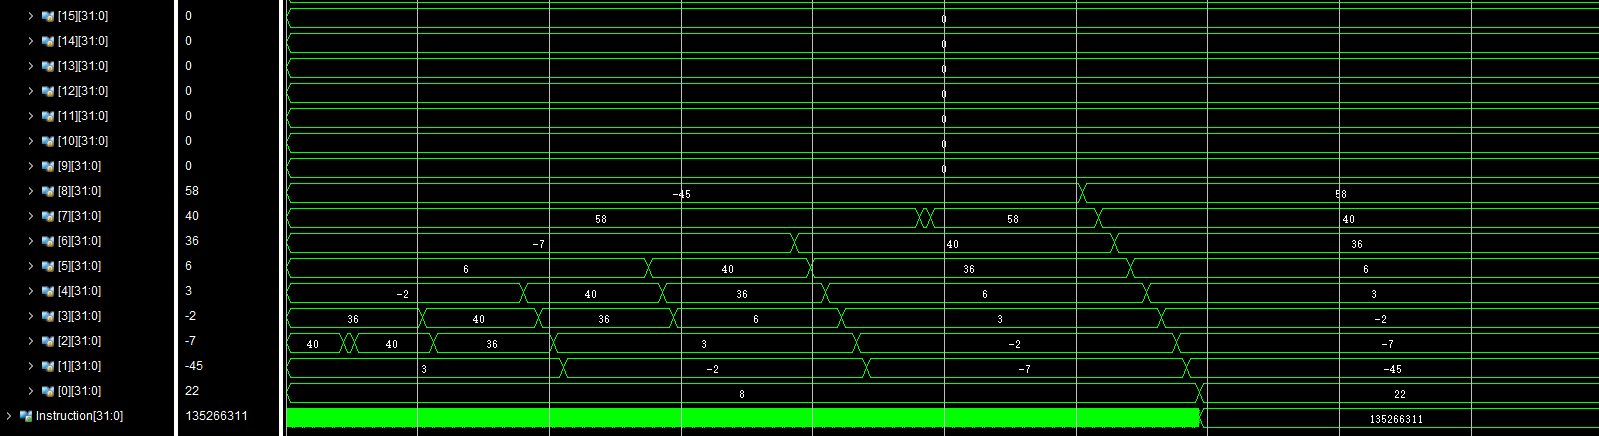
\includegraphics[scale=0.35]{sicy.png}
    \end{figure}
根据验收要求,进一步验证,对24个正整数排序如下:
\begin{figure}[H]
    \centering
    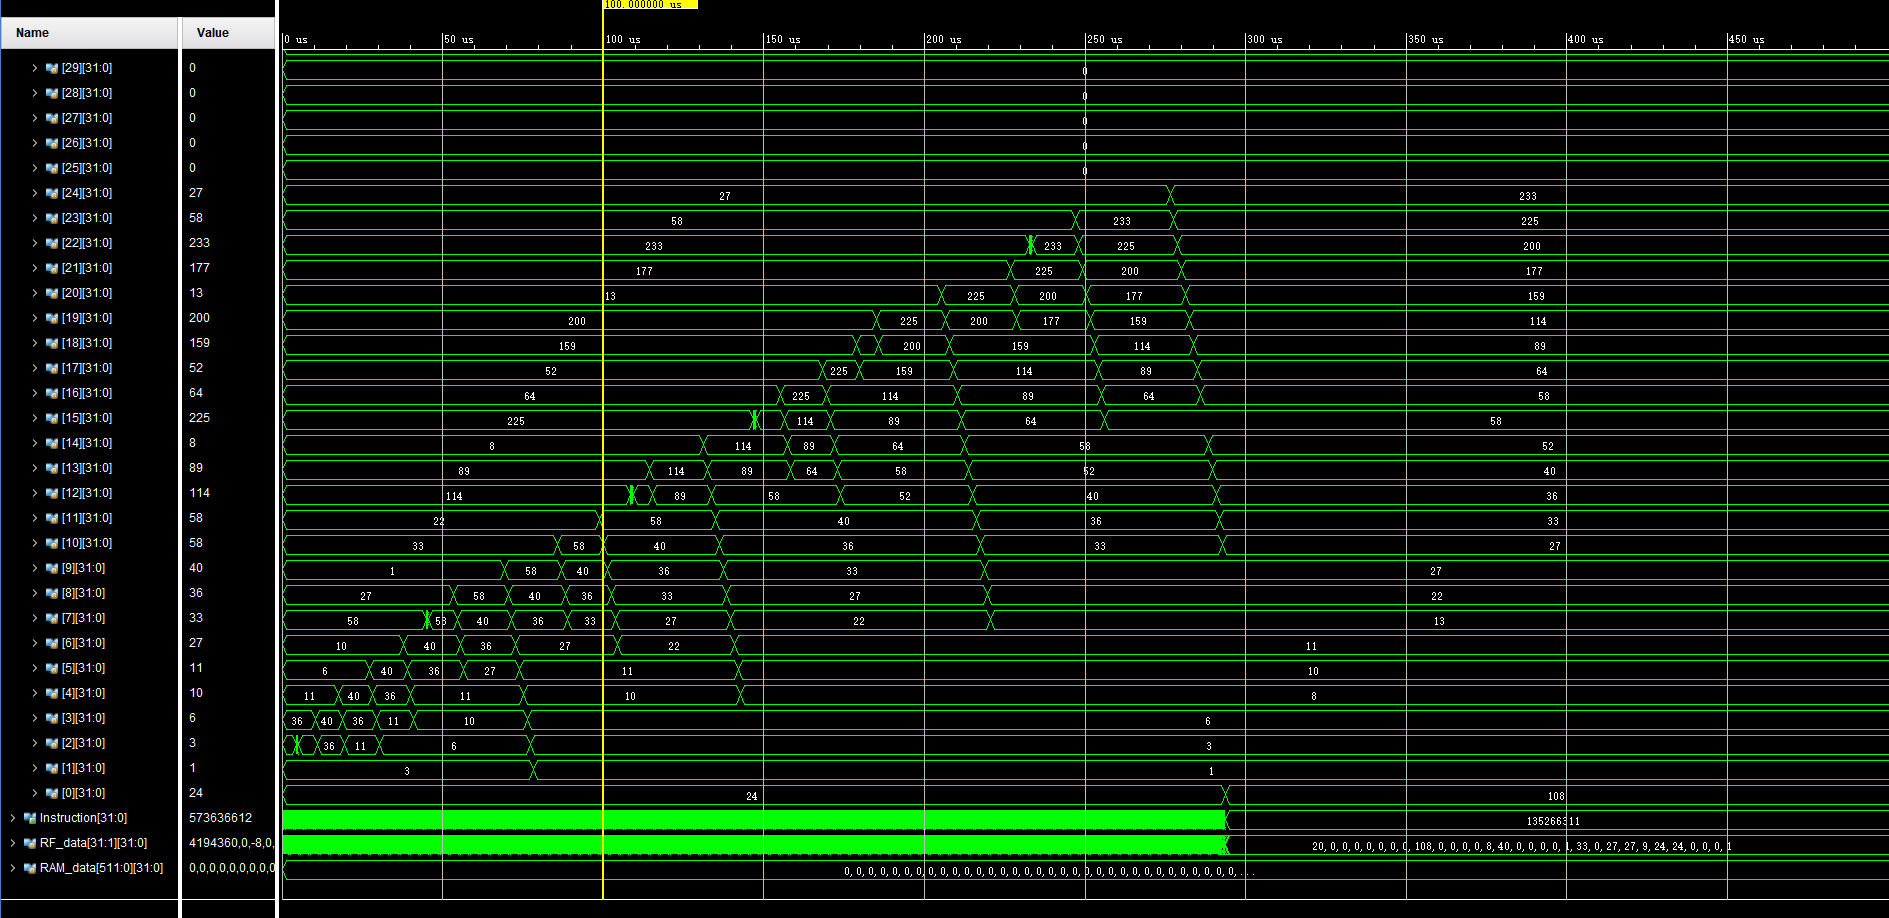
\includegraphics[scale=0.38]{MUCHOGUSTO.png}
    \end{figure}
\newpage
\section{流水线改造(无冒险处理)}
\begin{figure}[H]
    \centering
    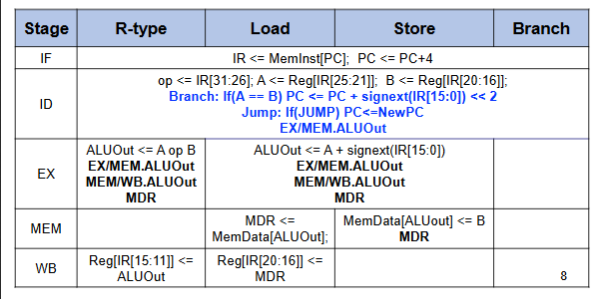
\includegraphics[scale=0.75]{table.png}
    \end{figure}
CPU.v的改动最大,需要在各模块输入/输出之间添加寄存器,以下
介绍寄存器的初步添加,不考虑冒险。

Control.v即控制信号模块在IF阶段调用,产生控制信号,为
传递控制信号,在CPU.v中插入IF/ID寄存器:
\begin{lstlisting}[style={verilog-style}]
	always @(posedge reset or posedge clk) begin//IF/ID PLUGIN BEGIN ↑IF
	   if (reset) begin
               IFID_Instruction <= 32'b0;
	       IFID_RegDst <= 2'b00;
	       IFID_PCSrc <= 2'b00;
	       IFID_Branch <= 3'b000;
	       IFID_MemRead <= 1'b0;
	       IFID_MemWrite <= 1'b0;
	       IFID_MemtoReg <= 2'b00;
	       IFID_ALUSrc1 <= 1'b0;
	       IFID_ALUSrc2 <= 1'b0;
	       IFID_ALUOp <= 4'b0000;
	       IFID_ExtOp <= 1'b0;
	       IFID_LuOp <= 1'b0;
	       IFID_RegWrite <= 1'b0;
	   end	   //more to consider
	   else begin
                IFID_Instruction <= Instruction;
	        IFID_RegDst <= RegDst;
                IFID_PCSrc <= PCSrc;
                IFID_Branch <= Branch;
                IFID_MemRead <= MemRead;
                IFID_MemWrite <= MemWrite;
                IFID_MemtoReg <= MemtoReg;
                IFID_ALUSrc1 <= ALUSrc1;
                IFID_ALUSrc2 <= ALUSrc2;
                IFID_ALUOp <= ALUOp;
                IFID_ExtOp <= ExtOp;
                IFID_LuOp <= LuOp;
                IFID_RegWrite <= RegWrite;
	   end
	end//IF/ID PLUGIN END ↓ID
\end{lstlisting}

ID阶段调用寄存器堆(读),注意WB阶段亦涉及调用寄存器堆(写),考虑
遵循先写后读原则(在RegisterFile.v中修改)。插入ID/EX寄存器:
\begin{lstlisting}[style={verilog-style}]

\end{lstlisting}

将Jump,Branch均置于ID阶段执行,则ALU不需要Zero。
无冒险处理的流水线例程测试如下:
\begin{figure}[H]
    \centering
    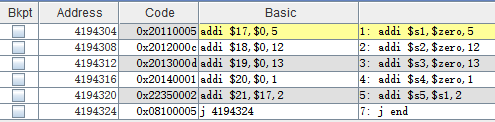
\includegraphics[scale=0.7]{hazardno.png}
\end{figure}
\begin{figure}[H]
    \centering
    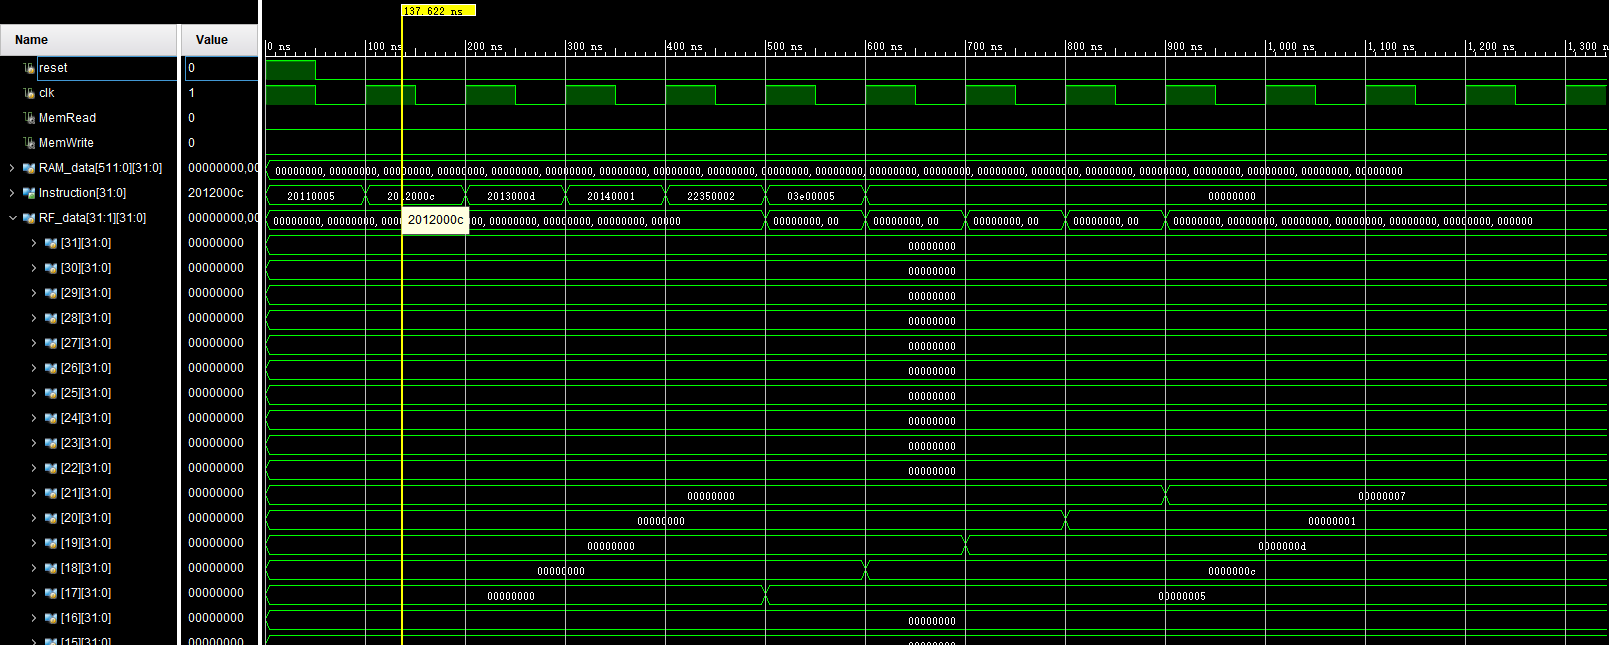
\includegraphics[scale=0.4]{norisk.png}
    \end{figure}
\newpage
\section{冒险处理}
\subsection{结构冒险}
InstructionMemory与DataMemory已作分离;R型指令
Mem阶段已空置;ALU已作功能疏解。
\subsection{数据冒险}
\subsubsection{同时读写寄存器堆}
\begin{figure}[H]
    \centering
    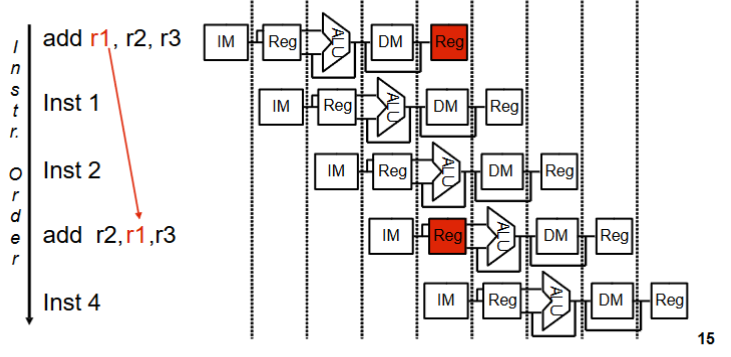
\includegraphics[scale=0.4]{reguse.png}
    \end{figure}

通过先写后读策略处理。利用always块的阻塞赋值实现代码执行的先后顺序。
\begin{lstlisting}[style={verilog-style}]
    always @(*) begin
        if (RegWrite && (Write_register != 5'b00000))
             RF_data[Write_register] = Write_data;//first write
        Read_data1 = (Read_register1 == 5'b00000)? 32'h00000000: RF_data[Read_register1];
        Read_data2 = (Read_register2 == 5'b00000)? 32'h00000000: RF_data[Read_register2];
    end
\end{lstlisting}
验证如下:
\begin{figure}[H]
    \centering
    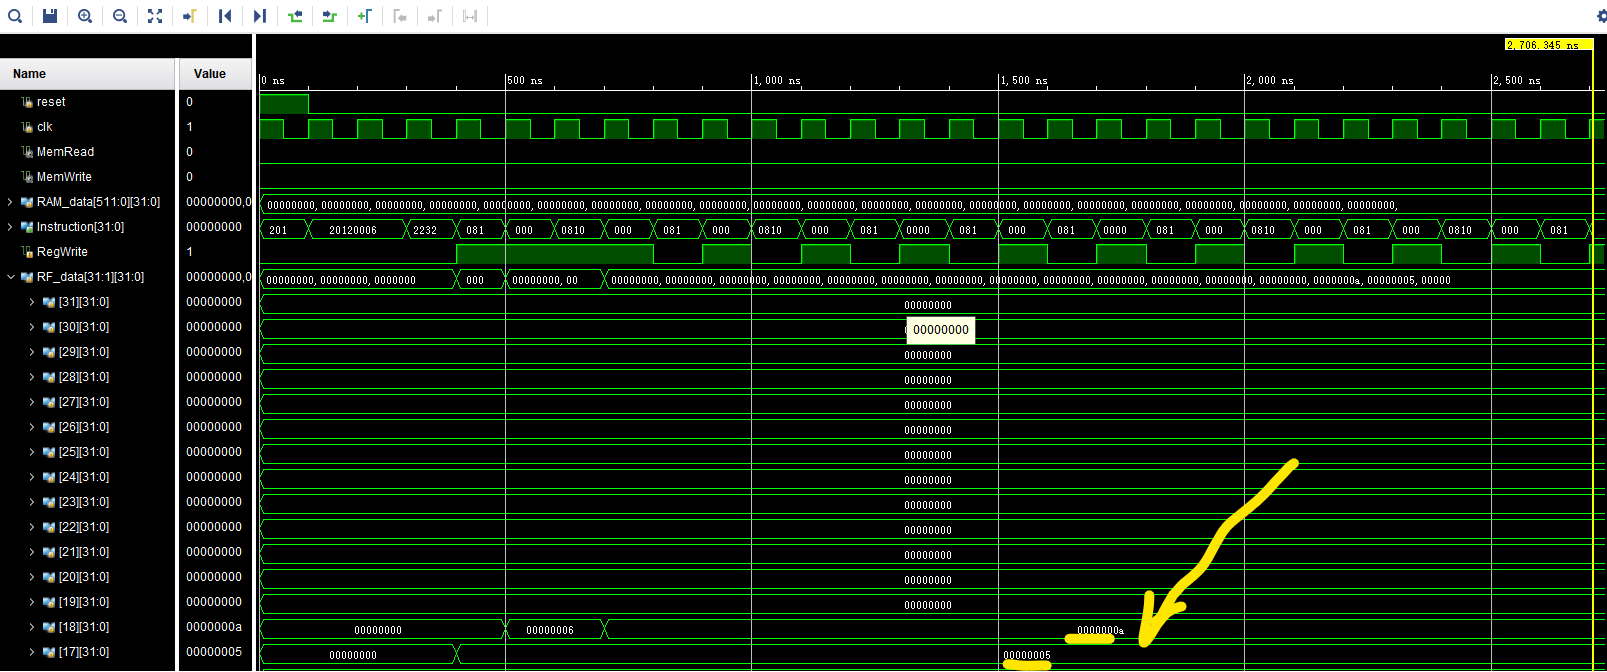
\includegraphics[scale=0.43]{fwtr.png}
    \end{figure}
    \begin{figure}[H]
        \centering
        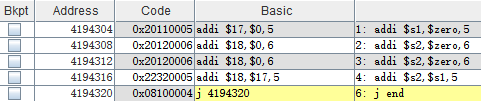
\includegraphics[scale=0.9]{fwtrx.png}
        \end{figure}
\subsubsection{时间顺序关联(ALU输出)}
\begin{figure}[H]
    \centering
    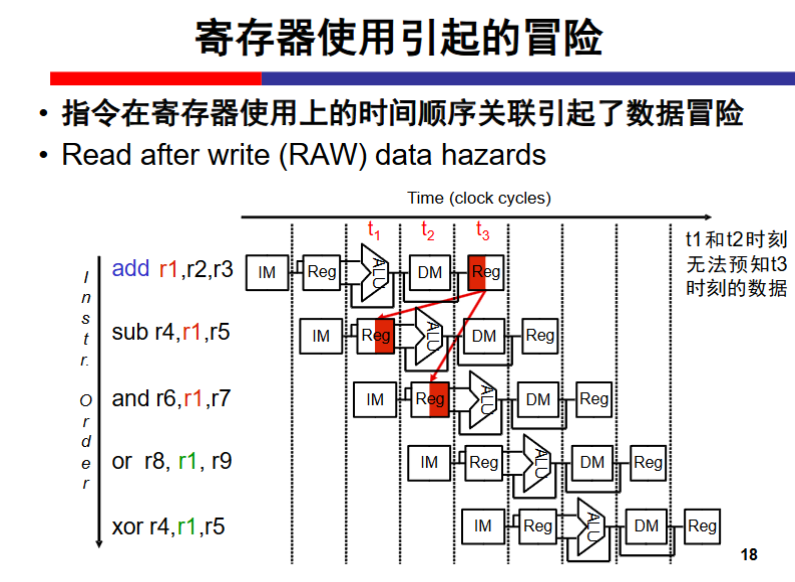
\includegraphics[scale=0.3]{reg.png}
    \end{figure}

ALU输出运算结果后,立刻转发给ALU输入端。需要修改ALU的输入端(二路),增加MUX选择合适的输入信号。
\begin{lstlisting}[style={verilog-style}]
    wire [32 -1:0] in1,in2;//rs,rt forwarding
    assign in1 = (~IDEX_ALUSrc1 && MEMWB_Memory_Read && MEMWB_Write_register 
        && MEMWB_Write_register == IDEX_Instruction[25:21])? MEMWB_MemBus_Read_Data:
        (~IDEX_ALUSrc1 && MEMWB_RegWrite && MEMWB_Write_register 
        && (MEMWB_Write_register == IDEX_Instruction[25:21])
        && (EXMEM_Write_register != IDEX_Instruction[25:21] 
        || ~EXMEM_RegWrite))? MEMWB_ALU_out:
        (~IDEX_ALUSrc1 && EXMEM_RegWrite && EXMEM_Write_register
        && (EXMEM_Write_register == IDEX_Instruction[25:21]))? EXMEM_ALU_out: 
        ALU_in1;
    assign in2 = (~IDEX_ALUSrc2 && MEMWB_Memory_Read && MEMWB_Write_register 
        && MEMWB_Write_register == IDEX_Instruction[20:16])? MEMWB_MemBus_Read_Data:
        (~IDEX_ALUSrc2 && MEMWB_RegWrite && MEMWB_Write_register 
        && (MEMWB_Write_register == IDEX_Instruction[20:16])
        && (EXMEM_Write_register != IDEX_Instruction[20:16] 
        || ~EXMEM_RegWrite))? MEMWB_ALU_out://mind load-store
        (~IDEX_ALUSrc2 && EXMEM_RegWrite && EXMEM_Write_register
        && (EXMEM_Write_register == IDEX_Instruction[20:16]))? EXMEM_ALU_out: 
        ALU_in2;
\end{lstlisting}
验证如下:
\begin{figure}[H]
    \centering
    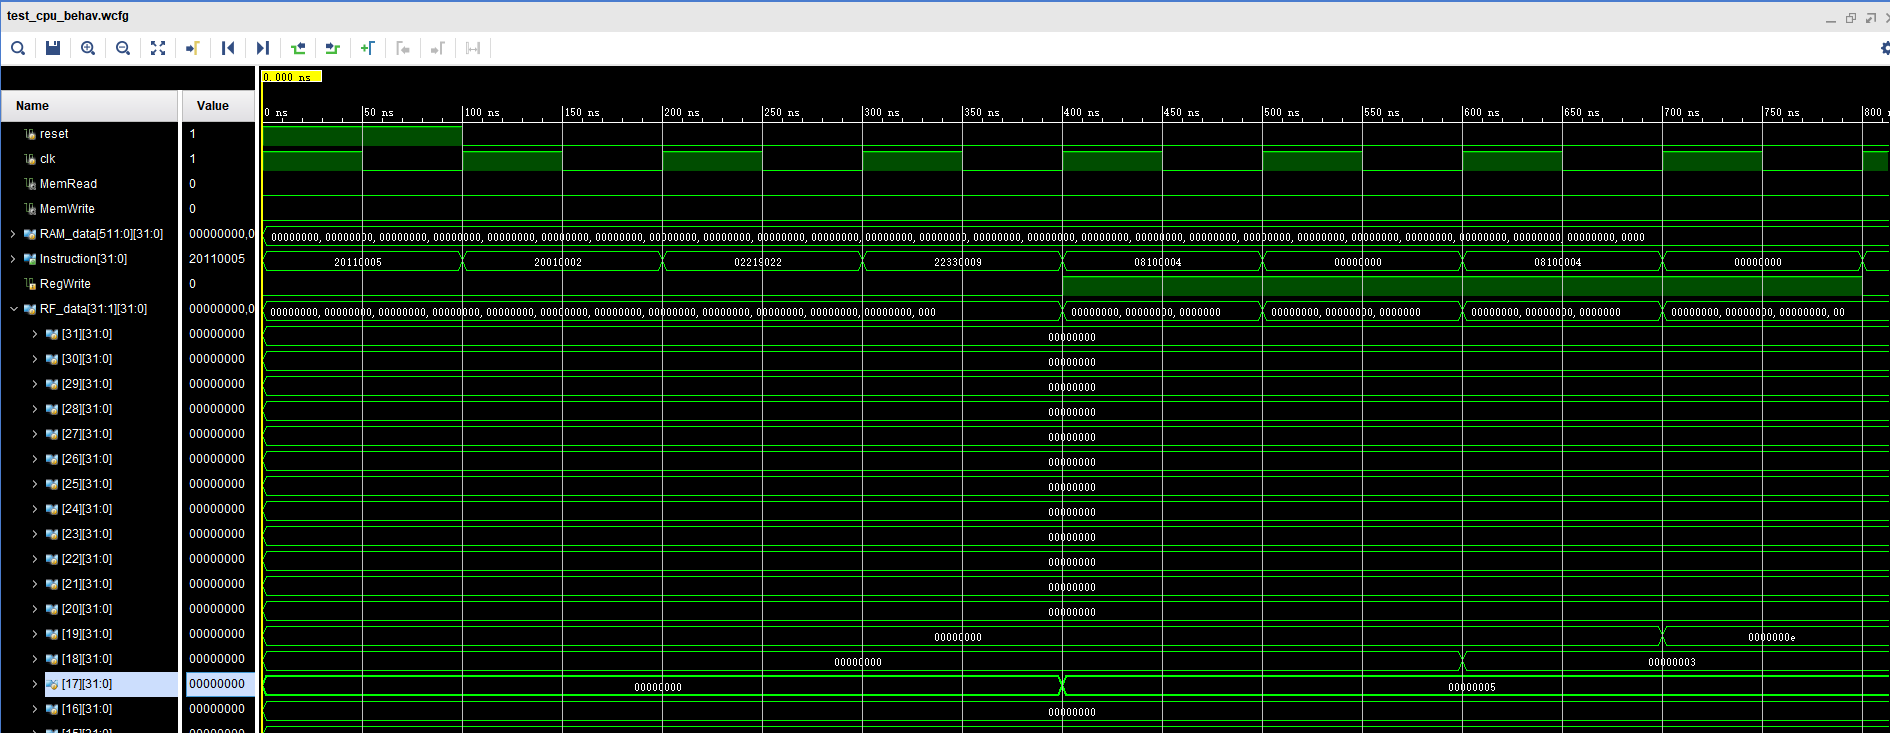
\includegraphics[scale=0.35]{haddaz.png}
    \end{figure}
    \begin{figure}[H]
        \centering
        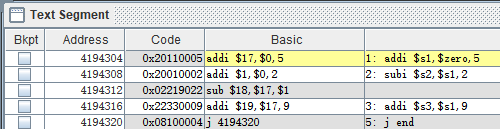
\includegraphics[scale=0.9]{hadd.png}
        \end{figure}
此外,若下一条指令为Branch(为简便,默认jr,jalr使用\$31,故不需要处理),
则不能不stall一个周期,再将数据转发到ID阶段。
验证如下:
\begin{figure}[H]
    \centering
    
\includegraphics[scale=0.4]{bgtzz.png}
    \end{figure}
    \begin{figure}[H]
        \centering
        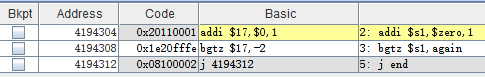
\includegraphics[scale=0.9]{bgtz.png}
        \end{figure}
\subsubsection{load-use冒险}
\begin{figure}[H]
    \centering
    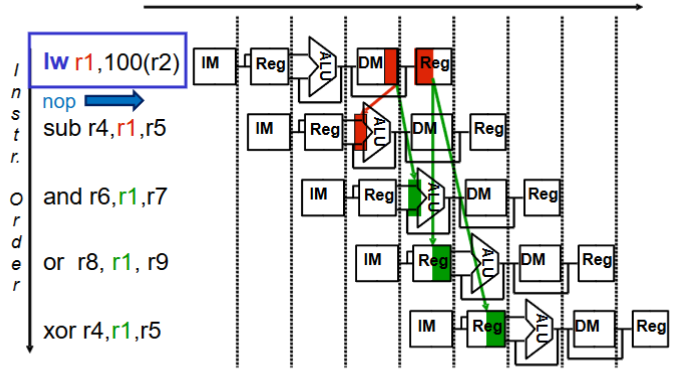
\includegraphics[scale=0.6]{load.png}
    \end{figure}
load-use冒险包含load-R类和load-store类冒险,前者不可避免地需要stall一个周期。
故需要将读出数据作转发。
处理load-store冒险时,在ALU输入forwarding条件中需要分辨立即数加法与寄存值加法;
DataMemory写端口也需要引入MUX作forwarding判断。

非常特殊的情况:
lw \$s1,4(\$zero),sw \$s1,0(\$s1),由于stall一个周期,无法由MEM/WB转发,同时\$s1尚未
更新。故需要特殊处理:
\begin{lstlisting}[style={verilog-style}]
    assign IDEX_Databus2_prevent_loadstore = (IDEX_MemWrite && MEMWB_Write_register
        && (MEMWB_Write_register == IDEX_Instruction[20:16]))? MEMWB_MemBus_Read_Data:
        IDEX_Databus2;
\end{lstlisting}
一般load-use处理效果如下:
\begin{figure}[H]
    \centering
    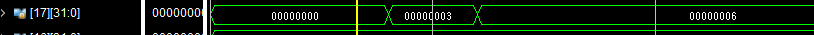
\includegraphics[scale=0.6]{add.png}
    \end{figure}
    \begin{figure}[H]
        \centering
        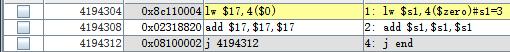
\includegraphics[scale=0.9]{addon.png}
        \end{figure}
一般load-store处理效果如下:
\begin{figure}[H]
    \centering
    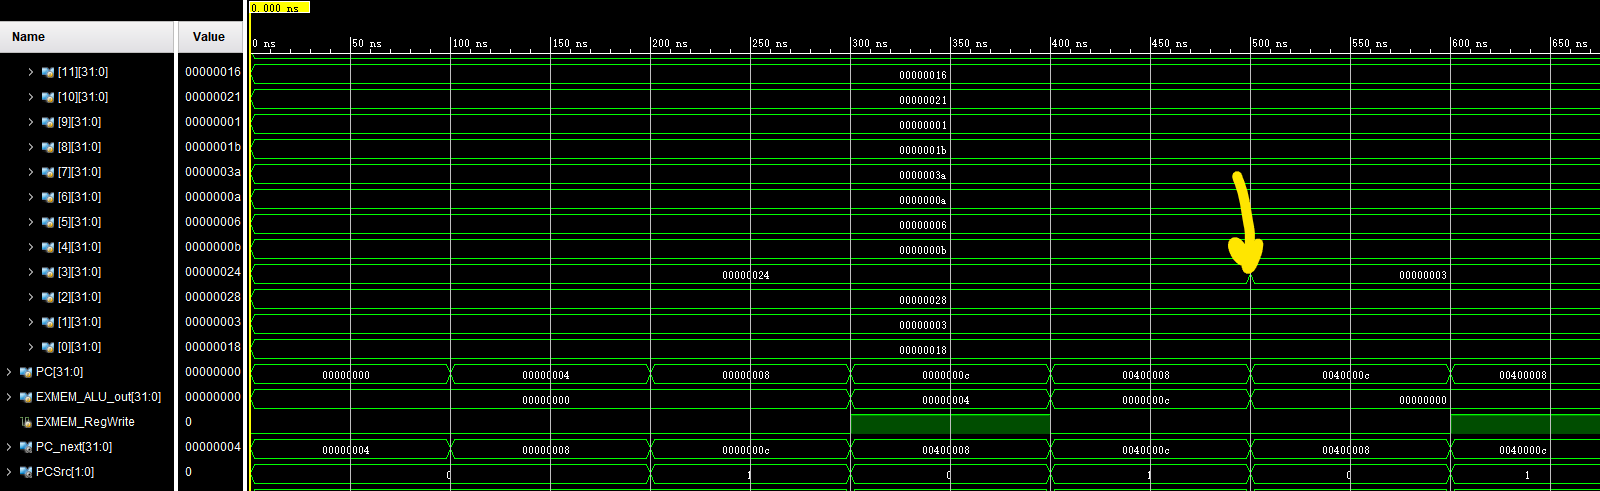
\includegraphics[scale=0.4]{lstore.png}
    \end{figure}
    \begin{figure}[H]
        \centering
        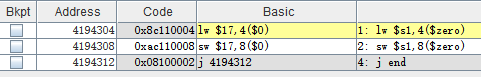
\includegraphics[scale=0.9]{fo.png}
        \end{figure}
特殊load-store处理效果如下:
\begin{figure}[H]
    \centering
    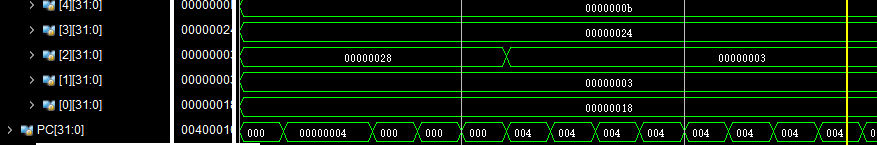
\includegraphics[scale=0.5]{specialls.png}
    \end{figure}
\begin{figure}[H]
    \centering
    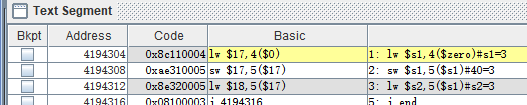
\includegraphics[scale=0.9]{hdl.png}
    \end{figure}

    另外,load后若紧跟Branch指令且发生冒险,则需要stall两个周期,
    暂不作处理,通过代码添加3个nop指令(0x00000000)解决。

    至此,数据冒险基本解决。
\subsection{控制冒险}
由于提前到ID阶段判断,分支指令、跳跃指令的下一条指令必然为nop。据此设定
修改即可。

利用流水线处理器排序结果如下:
\begin{figure}[H]
    \centering
    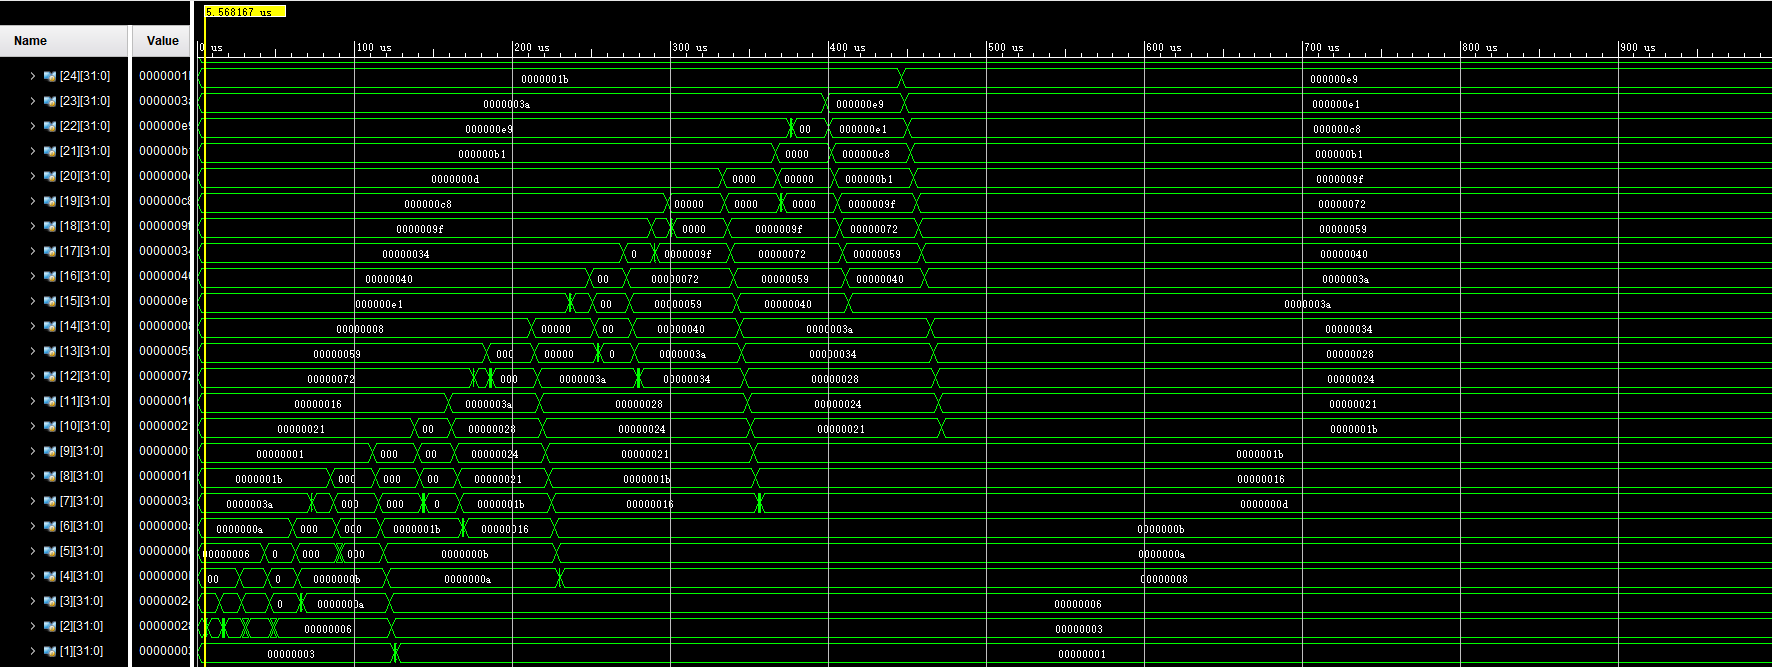
\includegraphics[scale=0.3]{mult.png}
    \end{figure}

\section{外设配置}

\end{document}










